% \section{Results}
% \label{sec:results}

\textbf{Simulation Results.}
We evaluate the simulation fidelity using the \gls{mse} averaged across all steps of a complete rollout, on a test split whose physical properties and initial conditions are unseen during training.
Figure~\ref{fig:main_results} shows that \gls{peach} outperforms the other learned point cloud encoders by a substantial margin.
It also outperforms the mesh-based \gls{mango} on three out of four environments despite its privileged mesh context, which we attribute to the limited capacity of the shallow \gls{cnn} and Deep Sets encoder of \gls{mango}.
\textit{Test-Time Optimization} is considerably less accurate than \gls{peach} on \texttt{Deforming Block} and on par on \texttt{Trampoline}, but matches the \textit{Oracle} on \texttt{Sheet Deformation} and achieves the lowest error on \texttt{Bending Beam}, at about $140$ times the inference time of \gls{peach} (Appendix~\ref{sec:runtime}).
On \texttt{Bending Beam}, both \textit{Test-Time Optimization} and \gls{peach} surpass the \textit{Oracle}.
We attribute this to approximation errors of the learned simulator.
Since both methods infer their conditioning from observed deformations, they can compensate for such errors by representing an effective stiffness that reproduces the observed bending, even if it deviates from the true material parameters, whereas the \textit{Oracle} is bound to the ground truth parameters.
\textit{Test-Time Optimization} performs this adaptation explicitly for each task, which explains its larger gain on the clean simulated observations.
Replacing the simulator with the step-based \gls{mgn} generally reduces accuracy, even with oracle information.
Figure~\ref{fig:task_overview} shows qualitative predictions of \gls{peach} across all four scenes, and Appendix~\ref{app:vis} provides additional qualitative results.

\textbf{Real World Results.}
Figure~\ref{fig:realworld_setup} shows an example trajectory of our real-world \texttt{Trampoline} setup. 
A robot arm releases a ball of unknown size and weight above an elastic membrane of varying thickness.
Figure~\ref{fig:qualitative_realworld} demonstrates that \gls{peach} is able to adapt to contexts from this real world setup without ever having seen real-world point clouds during training.
Qualitatively, \gls{peach} adapts to the interaction dynamics determined by the ball's size and weight and the rubber sheet's thickness, accurately capturing the sheet deformation at peak elongation.
In contrast, the \textit{No Context Encoding} baseline regresses to the mean, predicting only minimal deformation regardless of the physical parameters.

Quantitatively, \gls{peach} outperforms all baselines, including the \textit{Oracle} with material parameters measured directly from the physical setup and \textit{Test-Time Optimization}, whose accuracy degrades on the noisy and partially occluded real-world observations.
All methods perform well prior to ball-sheet contact, having learned to accurately predict free-fall dynamics, but baselines deteriorate significantly during the contact phase. 
Toward the end of the trajectory, prediction error increases across all methods, which we attribute to the inherently chaotic post-bounce behavior of the ball, whose direction after impact is difficult to predict deterministically.
Combined, these results indicate our method's ability to accurately simulate real-world scenes from only point cloud observations.

\begin{figure}[t]
    \makebox[\textwidth][c]{
        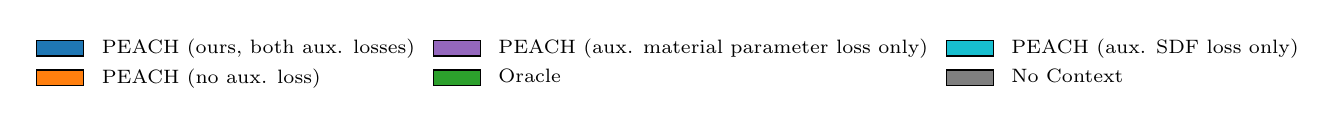
\begin{tikzpicture}
    \tikzstyle{every node}=[font=\scriptsize]
    \definecolor{tabblue}{RGB}{31, 119, 180}
\definecolor{taborange}{RGB}{255, 127, 14}
\definecolor{tabgreen}{RGB}{44, 160, 44}
\definecolor{tabred}{RGB}{214, 39, 40}
\definecolor{tabpurple}{RGB}{148, 103, 189}
\definecolor{tabbrown}{RGB}{140, 86, 75}
\definecolor{tabpink}{RGB}{227, 119, 194}
\definecolor{tabgray}{RGB}{127, 127, 127}
\definecolor{tabolive}{RGB}{188, 189, 34}
\definecolor{tabcyan}{RGB}{23, 190, 207}
\definecolor{ForestGreen}{RGB}{34, 139, 34}

    \begin{axis}[%
        hide axis,
        xmin=10,
        xmax=50,
        ymin=0,
        ymax=0.1,
        legend style={
            draw=none,
            legend cell align=left,
            legend columns=3,
            column sep=1ex,
        }
    ]

    % --- Bar-style legend entries ---
    \addlegendimage{area legend, fill=tabblue}
    \addlegendentry{PEACH (ours, both aux. losses)}

    \addlegendimage{area legend, fill=tabpurple}
    \addlegendentry{PEACH (aux. material parameter loss only)}

    \addlegendimage{area legend, fill=tabcyan}
    \addlegendentry{PEACH (aux. SDF loss only)}

    \addlegendimage{area legend, fill=taborange}
    \addlegendentry{PEACH (no aux. loss)}

    
    \addlegendimage{area legend, fill=tabgreen}
    \addlegendentry{Oracle}

    
    \addlegendimage{area legend, fill=tabgray}
    \addlegendentry{No Context}



    \end{axis}
\end{tikzpicture}
    }
  \centering
     \begin{minipage}{0.32\textwidth}
        \scalebox{0.6}{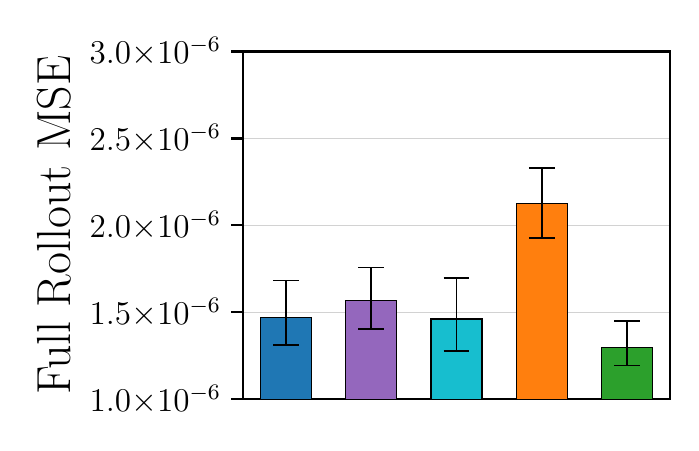
\begin{tikzpicture}
\definecolor{darkgray}{RGB}{169,169,169}
\definecolor{lightgray204}{RGB}{204,204,204}
\definecolor{tabblue}{RGB}{31,119,180}
\definecolor{taborange}{RGB}{255,127,14}
\definecolor{tabpurple}{RGB}{148,103,189}
\definecolor{tabred}{RGB}{214,39,40}
\definecolor{tabcyan}{RGB}{23,190,207}
\definecolor{tabgreen}{RGB}{44,160,44}

\begin{axis}[
    line width=0.8pt,
    axis line style={black},
    height=6cm,
    width=7cm,
    scaled y ticks=false,
    xmin=-0.5, xmax=4.5,
    xtick=\empty,
    ymin=1.0e-6, ymax=3.0e-6,
    ymajorgrids,
    y grid style={lightgray!70},
    tick align=outside,
    ylabel={Full Rollout MSE},
    ylabel style={font=\LARGE, color=black},
    tick label style={font=\large, color=black},
    ytick style={color=black, line width=0.8pt},
    ytick={1.0e-6, 1.5e-6, 2.0e-6, 2.5e-6, 3.0e-6},
    yticklabels={
        \(1.0{\times}10^{-6}\),
        \(1.5{\times}10^{-6}\),
        \(2.0{\times}10^{-6}\),
        \(2.5{\times}10^{-6}\),
        \(3.0{\times}10^{-6}\)
    },
    ytick pos=left,
]

% 0: pointpatch (tab:blue)
\draw[fill=tabblue, draw=black, line width=0.5pt]
    (axis cs:-0.3, 1e-6) rectangle (axis cs:0.3, 1.4707e-6);
% 1: peach_only_ml_and_matprop (tab:purple)
\draw[fill=tabpurple, draw=black, line width=0.5pt]
    (axis cs:0.7, 1e-6) rectangle (axis cs:1.3, 1.5698e-6);
% 2: peach_only_ml_and_sdf (tab:red)
\draw[fill=tabcyan, draw=black, line width=0.5pt]
    (axis cs:1.7, 1e-6) rectangle (axis cs:2.3, 1.4608e-6);
% 3: peach_only_ml (tab:orange)
\draw[fill=taborange, draw=black, line width=0.5pt]
    (axis cs:2.7, 1e-6) rectangle (axis cs:3.3, 2.1269e-6);
% 4: oracle (tab:green)
\draw[fill=tabgreen, draw=black, line width=0.5pt]
    (axis cs:3.7, 1e-6) rectangle (axis cs:4.3, 1.2985e-6);

% Error bars
% 0: pointpatch
\draw[black, semithick] (axis cs:0, 1.3136e-6) -- (axis cs:0, 1.6826e-6);
\draw[black, semithick] (axis cs:-0.15, 1.3136e-6) -- (axis cs:0.15, 1.3136e-6);
\draw[black, semithick] (axis cs:-0.15, 1.6826e-6) -- (axis cs:0.15, 1.6826e-6);
% 1: peach_only_ml_and_matprop
\draw[black, semithick] (axis cs:1, 1.4025e-6) -- (axis cs:1, 1.7580e-6);
\draw[black, semithick] (axis cs:0.85, 1.4025e-6) -- (axis cs:1.15, 1.4025e-6);
\draw[black, semithick] (axis cs:0.85, 1.7580e-6) -- (axis cs:1.15, 1.7580e-6);
% 2: peach_only_ml_and_sdf
\draw[black, semithick] (axis cs:2, 1.2787e-6) -- (axis cs:2, 1.6967e-6);
\draw[black, semithick] (axis cs:1.85, 1.2787e-6) -- (axis cs:2.15, 1.2787e-6);
\draw[black, semithick] (axis cs:1.85, 1.6967e-6) -- (axis cs:2.15, 1.6967e-6);
% 3: peach_only_ml
\draw[black, semithick] (axis cs:3, 1.9261e-6) -- (axis cs:3, 2.3300e-6);
\draw[black, semithick] (axis cs:2.85, 1.9261e-6) -- (axis cs:3.15, 1.9261e-6);
\draw[black, semithick] (axis cs:2.85, 2.3300e-6) -- (axis cs:3.15, 2.3300e-6);
% 4: oracle
\draw[black, semithick] (axis cs:4, 1.1949e-6) -- (axis cs:4, 1.4497e-6);
\draw[black, semithick] (axis cs:3.85, 1.1949e-6) -- (axis cs:4.15, 1.1949e-6);
\draw[black, semithick] (axis cs:3.85, 1.4497e-6) -- (axis cs:4.15, 1.4497e-6);

\end{axis}
\end{tikzpicture}}\\
        {\small \hspace*{18mm} \texttt{Deforming Block}}
     \end{minipage}
     \hspace{4mm}
     \begin{minipage}{0.32\textwidth}
        \scalebox{0.6}{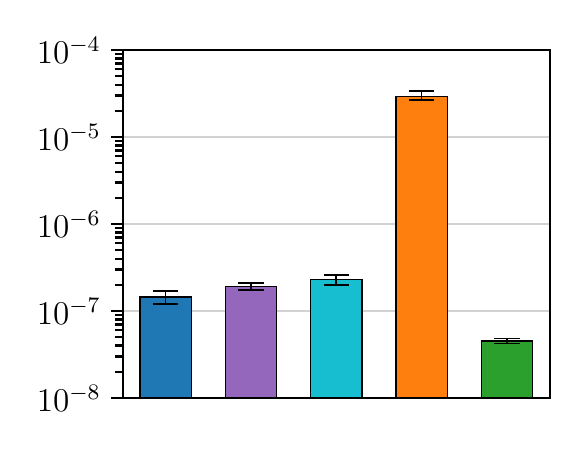
\begin{tikzpicture}
\definecolor{lightgray204}{RGB}{204,204,204}
\definecolor{tabblue}{RGB}{31,119,180}
\definecolor{taborange}{RGB}{255,127,14}
\definecolor{tabpurple}{RGB}{148,103,189}
\definecolor{tabred}{RGB}{214,39,40}
\definecolor{tabcyan}{RGB}{23,190,207}
\definecolor{tabgreen}{RGB}{44,160,44}

\begin{semilogyaxis}[
    line width=0.8pt,
    axis line style={black},
    height=6cm,
    width=7cm,
    xmin=-0.5, xmax=4.5,
    xtick=\empty,
    ymin=1e-8, ymax=1e-4,
    ymajorgrids,
    y grid style={lightgray!70},
    tick align=outside,
    % ylabel={Full Rollout MSE},
    ylabel style={font=\LARGE, color=black},
    tick label style={font=\large, color=black},
    ytick style={color=black, line width=0.8pt},
    ytick={1e-8, 1e-7, 1e-6, 1e-5, 1e-4},
    yticklabels={
        \(10^{-8}\),
        \(10^{-7}\),
        \(10^{-6}\),
        \(10^{-5}\),
        \(10^{-4}\)
    },
    ytick pos=left,
]

% Bars (bottom anchored at ymin=1e-8)
% 0: pointpatch (tab:blue)
\draw[fill=tabblue, draw=black, line width=0.5pt]
    (axis cs:-0.3, 1e-8) rectangle (axis cs:0.3, 1.4541e-7);
% 1: peach_only_ml_and_matprop (tab:purple)
\draw[fill=tabpurple, draw=black, line width=0.5pt]
    (axis cs:0.7, 1e-8) rectangle (axis cs:1.3, 1.9139e-7);
% 2: peach_only_ml_and_sdf (tab:red)
\draw[fill=tabcyan, draw=black, line width=0.5pt]
    (axis cs:1.7, 1e-8) rectangle (axis cs:2.3, 2.2891e-7);
% 3: peach_only_ml (tab:orange)
\draw[fill=taborange, draw=black, line width=0.5pt]
    (axis cs:2.7, 1e-8) rectangle (axis cs:3.3, 2.9077e-5);
% 4: oracle (tab:green)
\draw[fill=tabgreen, draw=black, line width=0.5pt]
    (axis cs:3.7, 1e-8) rectangle (axis cs:4.3, 4.5173e-8);

% Error bars
% 0: pointpatch
\draw[black, semithick] (axis cs:0, 1.2069e-7) -- (axis cs:0, 1.6982e-7);
\draw[black, semithick] (axis cs:-0.15, 1.2069e-7) -- (axis cs:0.15, 1.2069e-7);
\draw[black, semithick] (axis cs:-0.15, 1.6982e-7) -- (axis cs:0.15, 1.6982e-7);
% 1: peach_only_ml_and_matprop
\draw[black, semithick] (axis cs:1, 1.7561e-7) -- (axis cs:1, 2.0982e-7);
\draw[black, semithick] (axis cs:0.85, 1.7561e-7) -- (axis cs:1.15, 1.7561e-7);
\draw[black, semithick] (axis cs:0.85, 2.0982e-7) -- (axis cs:1.15, 2.0982e-7);
% 2: peach_only_ml_and_sdf
\draw[black, semithick] (axis cs:2, 1.9907e-7) -- (axis cs:2, 2.6067e-7);
\draw[black, semithick] (axis cs:1.85, 1.9907e-7) -- (axis cs:2.15, 1.9907e-7);
\draw[black, semithick] (axis cs:1.85, 2.6067e-7) -- (axis cs:2.15, 2.6067e-7);
% 3: peach_only_ml
\draw[black, semithick] (axis cs:3, 2.6516e-5) -- (axis cs:3, 3.3661e-5);
\draw[black, semithick] (axis cs:2.85, 2.6516e-5) -- (axis cs:3.15, 2.6516e-5);
\draw[black, semithick] (axis cs:2.85, 3.3661e-5) -- (axis cs:3.15, 3.3661e-5);
% 4: oracle
\draw[black, semithick] (axis cs:4, 4.2259e-8) -- (axis cs:4, 4.8071e-8);
\draw[black, semithick] (axis cs:3.85, 4.2259e-8) -- (axis cs:4.15, 4.2259e-8);
\draw[black, semithick] (axis cs:3.85, 4.8071e-8) -- (axis cs:4.15, 4.8071e-8);

\end{semilogyaxis}
\end{tikzpicture}}\\
        {\small \hspace*{8mm}\texttt{Sheet Deformation}}
     \end{minipage}
     \hspace{-4mm}
    \begin{minipage}{0.32\textwidth}
        \centering
        \scalebox{0.6}{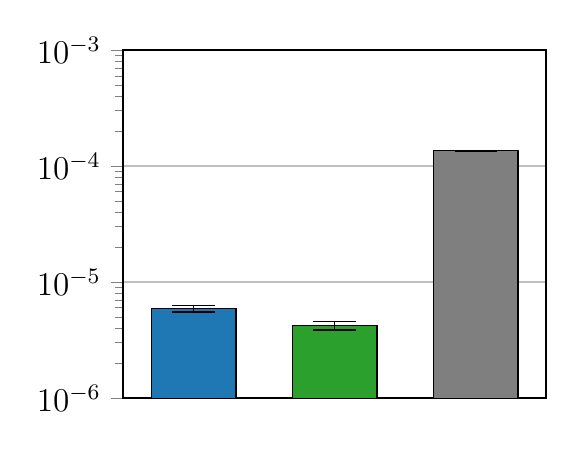
\begin{tikzpicture}
\definecolor{darkgray}{RGB}{169,169,169}
\definecolor{darkorange25512714}{RGB}{255,127,14}
\definecolor{darkslategray38}{RGB}{38,38,38}
\definecolor{darkturquoise23190207}{RGB}{23,190,207}
\definecolor{gray127}{RGB}{127,127,127}
\definecolor{lightgray204}{RGB}{204,204,204}
\definecolor{mediumpurple148103189}{RGB}{148,103,189}
\definecolor{orchid227119194}{RGB}{227,119,194}
\definecolor{sienna1408675}{RGB}{140,86,75}
\definecolor{steelblue31119180}{RGB}{31,119,180}
\definecolor{steelblue76114176}{RGB}{76,114,176}
\definecolor{tabgreen}{RGB}{44,160,44}

\begin{semilogyaxis}[
  line width=0.8pt,
  axis line style={black},
  xmin=-0.5, xmax=2.5,
  xtick=\empty,
  ymin=1e-6, ymax=1e-3,
  ymajorgrids,
  height=6cm,
  ytick pos=left,
  % width=7cm,
  % x grid style={lightgray204},
  % y grid style={lightgray204},
  % axis line style={darkgray},
  tick align=outside,
  % ylabel={Full Rollout MSE},
  ylabel style={font=\LARGE},
  tick label style={font=\large},
]

% Bars (bottom anchored at ymin=1e-7)
% 0: pointpatch (tab:blue)
\draw[fill=steelblue31119180, draw=black, line width=0.5pt] (axis cs:-0.3, 1e-7) rectangle (axis cs:0.3, 0.00000590559102420229);
% 1: oracle (tab:green)
\draw[fill=tabgreen, draw=black, line width=0.5pt] (axis cs:0.7, 1e-7) rectangle (axis cs:1.3, 0.00000421955195406554);
% 3: dummy (tab:gray)
\draw[fill=gray127, draw=black, line width=0.5pt] (axis cs:1.7, 1e-7) rectangle (axis cs:2.3, 0.000135723821585998);

% Error bars
% 0: pointpatch
\draw[black, semithick] (axis cs:0, 0.00000553021868654469
) -- (axis cs:0, 0.0000062809633618599);
\draw[black, semithick] (axis cs:-0.15, 0.00000553021868654469) -- (axis cs:0.15, 0.00000553021868654469);
\draw[black, semithick] (axis cs:-0.15, 0.0000062809633618599) -- (axis cs:0.15, 0.0000062809633618599);
% 1: oracle
\draw[black, semithick] (axis cs:1, 0.00000387946136015671) -- (axis cs:1, 0.00000455964254797436);
\draw[black, semithick] (axis cs:0.85, 0.00000387946136015671) -- (axis cs:1.15, 0.00000387946136015671);
\draw[black, semithick] (axis cs:0.85, 0.00000455964254797436) -- (axis cs:1.15, 0.00000455964254797436);
% 3: dummy
\draw[black, semithick] (axis cs:2, 0.000135091322590597) -- (axis cs:2, 0.000136356320581399);
\draw[black, semithick] (axis cs:1.85, 0.000135091322590597) -- (axis cs:2.15, 0.000135091322590597);
\draw[black, semithick] (axis cs:1.85, 0.000136356320581399) -- (axis cs:2.15, 0.000136356320581399);


\end{semilogyaxis}
\end{tikzpicture}}\\
        {\small \hspace*{4mm}\texttt{Deforming Block (OOD)}}
        
    \end{minipage}
  % 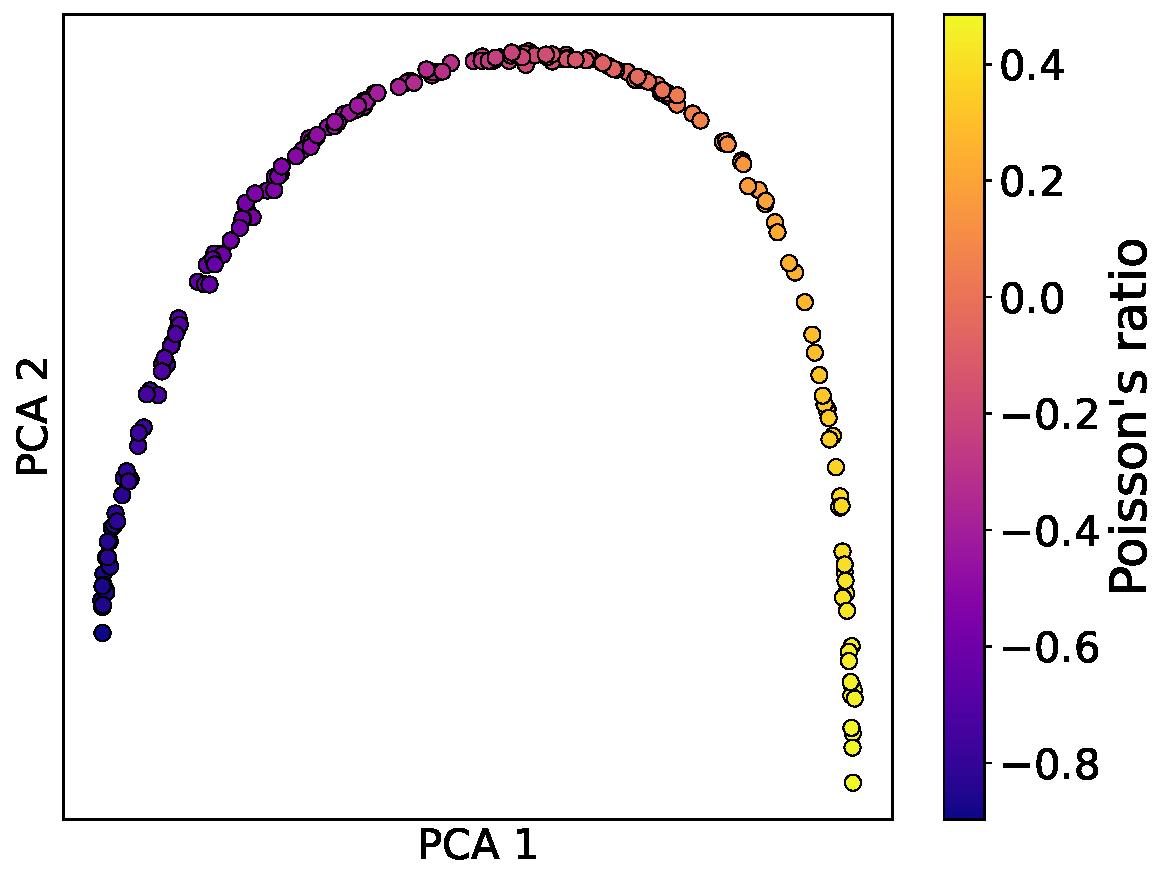
\includegraphics[width=0.33\textwidth]{figures/latent_space_vis/pca_peach_db_poisson.pdf}
  % 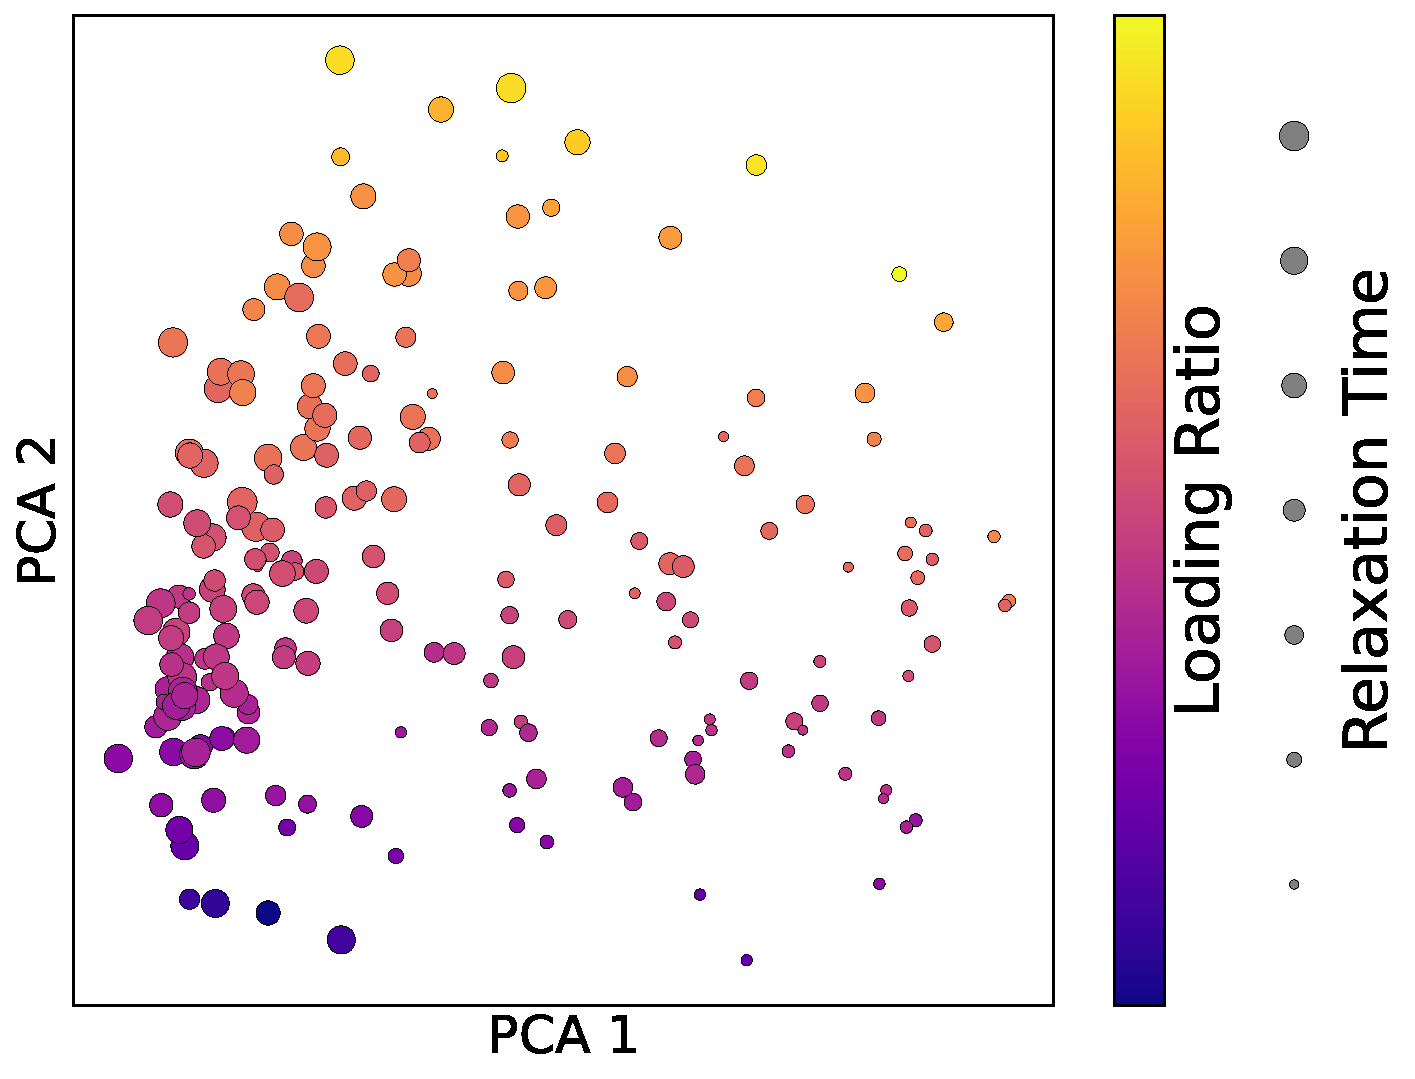
\includegraphics[width=0.33\textwidth]{figures/latent_space_vis/pca_peach_trampoline_bivariate.pdf}
  \caption{  \textbf{Left, Center:} Ablation study of auxiliary losses in PEACH on the
  \texttt{Deforming Block} and \texttt{Sheet Deformation} environments, respectively.
  \textbf{Right:} Performance of PEACH on out-of-distribution test tasks for
  \texttt{Deforming Block}.}
  \vspace{-0.4cm}
  \label{fig:generalizations_ablations}
\end{figure}

%PCA latent space visualization of all the Deforming Block dataset. Each dot is an encoded task, the color is its ground truth Poisson's ratio. Latent space visualizations of all further tasks are given in Appendix \todo{ref}.
\textbf{Parameter Study.}
We test the extrapolation capability of \gls{peach} using an additional, out-of-distribution set of \texttt{Deforming Block} tasks in simulation. As illustrated in Figure~\ref{fig:ood_split} of the Appendix, test tasks are drawn from the tails of the Poisson ratio distribution, ensuring that the evaluated material properties lie outside the training range.
% , where the Poisson's ratio values for test tasks are sampled outside the training distribution.
% Figure \ref{fig:generalizations_ablations} (right) further shows the out-of-distribution evaluation on \texttt{Deforming Block (OOD)}, where test tasks have Poisson's ratio values outside the training regime.
Figure \ref{fig:generalizations_ablations} (right) in the Appendix shows that \gls{peach} remains close to the oracle performance even under this distribution shift, demonstrating that the learned latent material representation generalizes beyond the training distribution.
A general analysis of performance as a function of context size is provided in Figure~\ref{fig:context_mse} of the Appendix~\ref{app:quant}.

\begin{wrapfigure}{r}{0.4\textwidth}
    \vspace{-0.4cm}
    \centering
    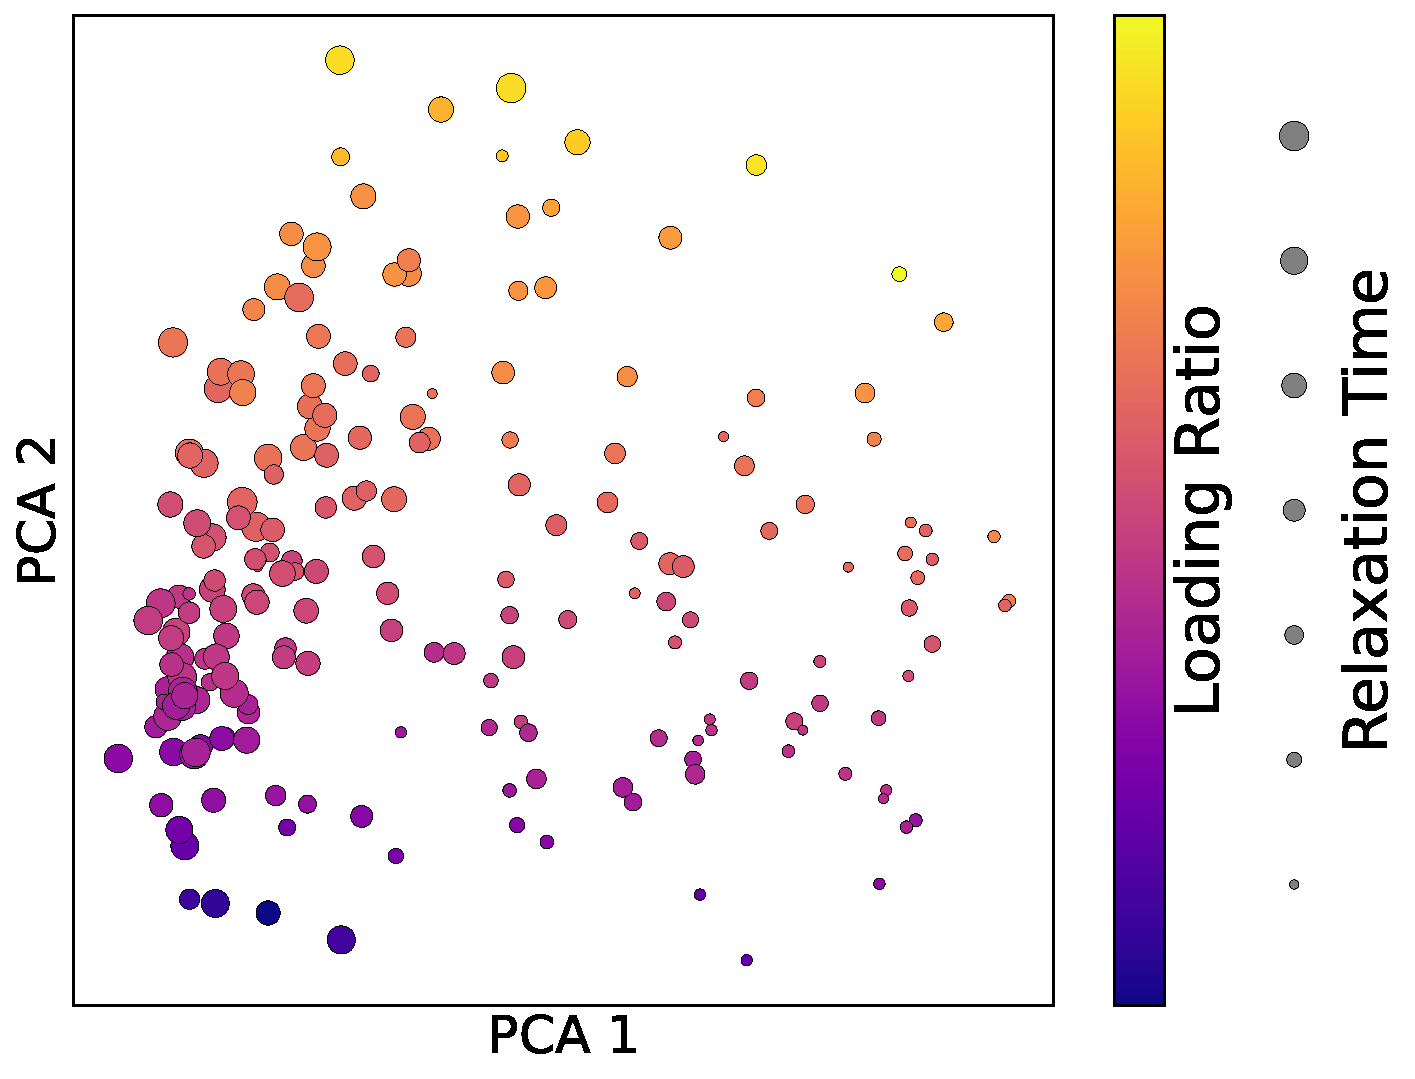
\includegraphics[width=\linewidth]{figures/latent_space_vis/pca_peach_trampoline_bivariate.pdf}
\caption{
    Visualization of the first and second PCA component of the latent space on the \texttt{Trampoline} dataset.
    Each point represents one simulation test task.
    Color corresponds to ratio of mass to product of Young's modulus and sheet thickness, i.e., loading ratio, which governs the degree of sheet deformation.
    Size corresponds to relaxation time.
    }
    \vspace{-0.4cm}
    \label{fig:latent_space_vis_main}
\end{wrapfigure}


\textbf{Ablations.}
Figure~\ref{fig:generalizations_ablations} (left, center) in the Appendix presents an ablation of the auxiliary losses on \texttt{Deforming Block} and \texttt{Sheet Deformation}.
Removing both auxiliary losses leads to a substantial performance drop, confirming that auxiliary supervision is critical for learning a useful latent material representation.
While \gls{peach} benefits from combining both losses, training with only the SDF auxiliary loss remains competitive.
Since \gls{sdf} labels can be computed purely from mesh geometry, this is a practical option for settings where ground truth physical properties are unavailable.
To test robustness to sensor artifacts, we corrupt the real-world context point clouds by removing $1\%$, $9\%$, or $25\%$ of the points in small patches and adding the same number of spurious points (Figure~\ref{fig:corruption} in Appendix~\ref{app:corruption}).
\gls{peach} remains nearly unaffected by all corruption levels and stays more accurate than the \textit{Oracle} during the contact phase.
Without data augmentation, its accuracy drops slightly on clean observations (Figure~\ref{fig:qualitative_realworld}, right) and considerably under high corruption, approaching the \textit{No Context} baseline at peak contact.


\textbf{Latent Space Analysis.}
Figure~\ref{fig:latent_space_vis_main} visualizes the PCA projection of the latent material codes encoded by \gls{peach} on the \texttt{Trampoline} dataset.
Despite no explicit structure being imposed on the latent space, the projection reveals a clear organization: the first principal component separates tasks by relaxation time, while the second separates them by loading ratio.
This emergent disentanglement of physically meaningful material properties suggests that \gls{peach} learns structured representations purely from point cloud observations. Latent space visualizations for all environments are provided in Figure~\ref{fig:latents_appendix} of the Appendix. A quantitative analysis in Appendix~\ref{app:latent_analysis} further shows that the variance of the latent description decreases with the context size at a rate close to averaging independent observations, and that distances between tasks in the latent space correlate strongly with distances between their physical parameters.


